\chapter{Simulation eines einfaches Multikoptermodell}\label{chap:simpleModel}
In der Literatur \cite{LQR2013}, \cite{mathModell} wird als passender physikalischer Ansatz die Newton'schen Bewegungsgleichungen und der Drallsatz verwendet. Der alternative Ansätze des Newton - Euler - Verfahren \cite[S. 36]{Sose2014} hatten sich als umständlich und analytisch aufwendig herausgestellt. \\

Der Multikopter lässt sich in drei Körpergruppen ($B_0, B_1, B_2$) einteilen: Bezugssystem (Startpunkt), ``nicht rotierende Körper'' (Grundplatte, Arme, Controller, Batterie, etc) und ``rotierende Körper'' (Motor, Rotor, Rotorschraube). In der Abbildung \ref{fig:schubkraefte} lassen sich die Schubkräfte $F_1, ... F_4$, wirkend im jeweiligen rotierenden System $B_{M1}, ..., B_{M2}$, erkennen. 
\begin{figure}[ht]
  \centering
  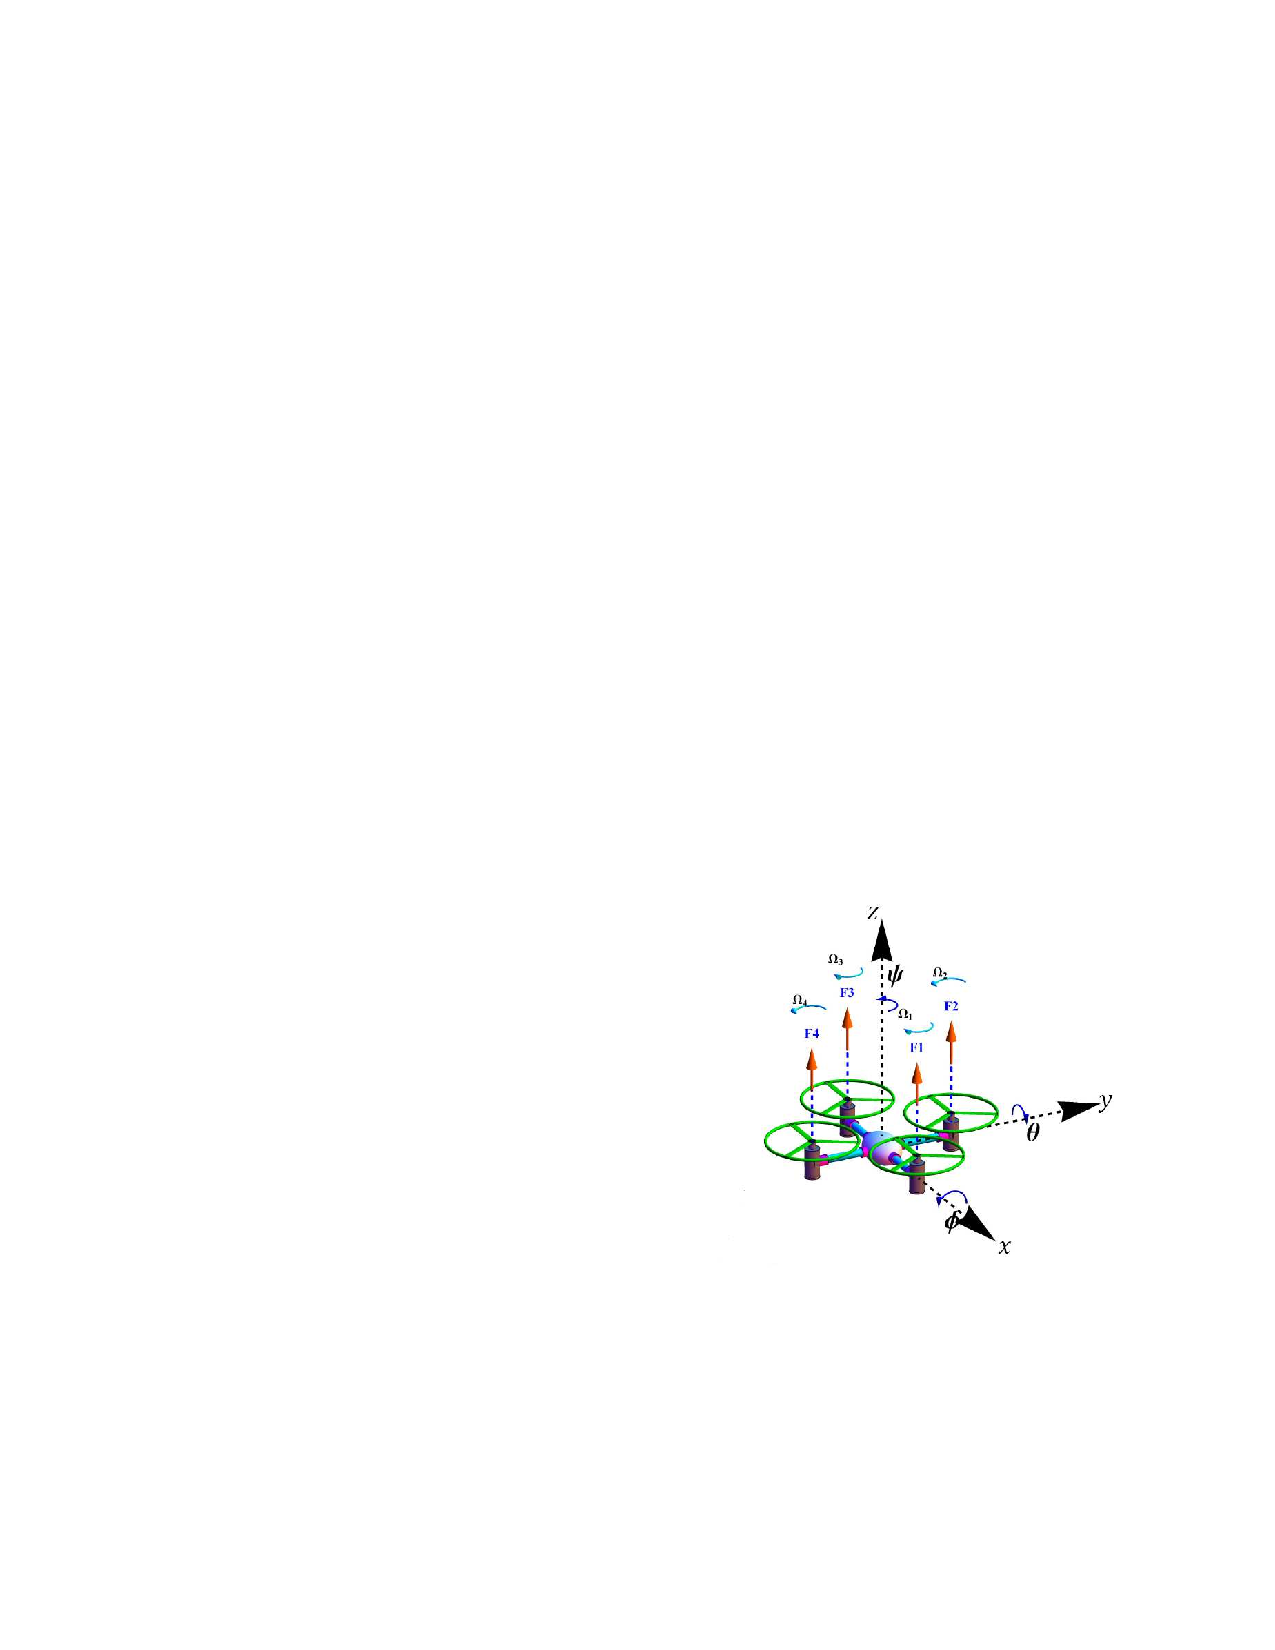
\includegraphics{images/MulticopterKraefte.pdf}
  \caption{Schubkräfte der Motoren}
  \label{fig:schubkraefte}
\end{figure}
Mit der, nicht eingezeichneten, Gewichtskraft führt dies zur folgenden Kräftegleichgewicht im KOS($B_0$).
\begin{align}
    \frac{d}{dt} F_{B_1} &= m_{B_1} \cdot \frac{d}{dt} {_{1}v_{1}} = m_{B_1} \frac{d_1}{dt} {_{1}v_{1}} + {_{1}\omega_{1}} \times m_{B_1} {_{1}v_{1}} \\
    &=  {_{1}F_g} + \sum_{i = 1}^{4}{_{1}F_{i}}  \\\notag
    &= m_{B_1} A_{1, 0} \cdot \begin{pmatrix} 0 \\ 0 \\ -g \end{pmatrix} + \sum_{i = 1}^4 {A_{1, M_i} \cdot _{M_i}F_{M_i}} \\
    &= m_{B_1} A_{1, 0} \cdot \begin{pmatrix} 0 \\ 0 \\ -g \end{pmatrix} + \sum_{i = 1}^4 {\begin{pmatrix} 0 \\ 0 \\ F_i \end{pmatrix}}
\end{align}

Dabei entspricht:\\
\begin{tabular}[t]{|l|l|}
  \hline
  $m_ges$ & Gesamtmasse des Multikopters \\ 
  $g$     & Gewichtskraft \\
  $A_{0,1}$ & Rotationsmatrix von Körper $B_1$ ins $B_0$ System \\
  $A_{1,M_i}$ & Rotationsmatrix von Körper $B_i$ ins $B_1$ System \\
  \hline
\end{tabular}\\

Die Rotationsmatrix $A_{1, M_i}$ ändert sich je nach Konfiguration des Multikopter. Die Abbildung \ref{fig:Konfigurationen} zeigt die behandele Konfiguration.
\begin{figure}[ht]
  \centering
  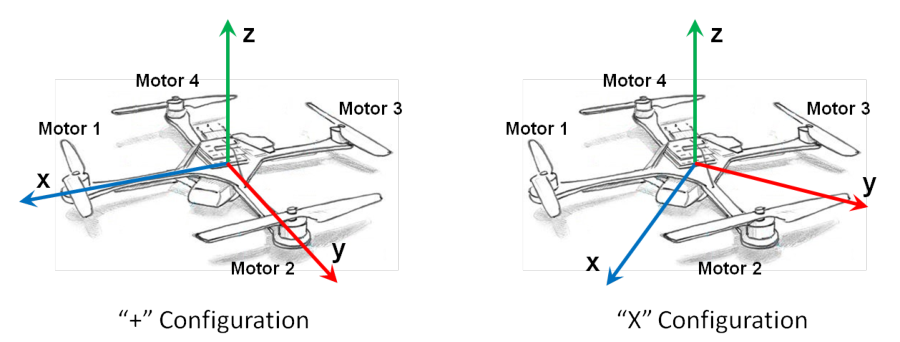
\includegraphics{images/Konfigurationen.pdf}
  \caption{Konfigurationen}
  \label{fig:Konfigurationen}
\end{figure}
\section{Konfigurationsmatrizen}\label{sec:konfg_matrix}
Für die ``+'' - Konfiguration werden folgende Matrizen verwendend:
\[
  A_{1, M_1} = \begin{pmatrix} 1 & 0 & 0 \\ 0 & 1 & 0 \\ 0 & 0 & 1 \end{pmatrix}
  A_{1, M_2} = \begin{pmatrix} 0 & -1 & 0 \\ 1 & 0 & 0 \\ 0 & 0 & 1 \end{pmatrix}
  A_{1, M_3} = \begin{pmatrix} -1 & 0 & 0 \\ 0 & -1 & 0 \\ 0 & 0 & 1 \end{pmatrix} 
  A_{1, M_4} = \begin{pmatrix} 0 & 1 & 0 \\ -1 & 0 & 0 \\ 0 & 0 & 1 \end{pmatrix}
\]
Für die ``x'' - Konfiguration werden folgende Matrizen verwendend:
\[
  A_{1, M_1} = \begin{pmatrix} \frac{\sqrt{2}}{2} & \frac{\sqrt{2}}{2} & 0 \\ \frac{-\sqrt{2}}{2} & \frac{\sqrt{2}}{2} & 0 \\ 0 & 0 & 1 \end{pmatrix} \hspace{0.5em}
  A_{1, M_2} = \begin{pmatrix} \frac{\sqrt{2}}{2} & -\frac{\sqrt{2}}{2} & 0 \\ \frac{\sqrt{2}}{2} & \frac{\sqrt{2}}{2} & 0 \\ 0 & 0 & 1 \end{pmatrix}
\]
\[
  A_{1, M_3} = \begin{pmatrix} -\frac{\sqrt{2}}{2} & -\frac{\sqrt{2}}{2} & 0 \\ \frac{\sqrt{2}}{2} & -\frac{\sqrt{2}}{2} & 0 \\ 0 & 0 & 1 \end{pmatrix} \hspace{0.5em}
  A_{1, M_4} = \begin{pmatrix} -\frac{\sqrt{2}}{2} & \frac{\sqrt{2}}{2} & 0 \\ -\frac{\sqrt{2}}{2} & -\frac{\sqrt{2}}{2} & 0 \\ 0 & 0 & 1 \end{pmatrix}
\]
\section{Mathematisches Modell}
Für Kräftegleichgewicht sind die Matrizen nicht relevant aber für den nach folgende Drallsatz im körperfesten System $B_1$. %Zuvor wird der Drallsatz im körperfesten System der Motoren betrachtet. Dort wirkt dem Drehmoment der Motoren $M_i$ ein Reaktionsdrehmoment  $\tau_i$ entgegen:
Zuvor wird aber zunächst ein festmontierter Motor betrachtet mit Drehmoment $M$. Diesem wirkt ein Strömungswiderstand $\tau_{drag}$ entgegen und es gilt: 
\begin{align}
{I_{rot}} \cdot \dot{\omega}  = M - \tau_{drag} 
\end{align}

Dabei ist $I_{rot}$ das Trägheitsmoment des Rotor endlang seiner z-Achse. Der Strömungswiderstand ist in der Literatur folgenderweise definiert als:
\begin{align}
    \tau_{drag} = \frac{1}{2} \rho A_r v^2
\end{align}
$\rho$ ist die Luftdichte, $A_r$ die Fläche, die der Rotor bei der Umdrehung überschreitet und $v$ ist die Geschwindigkeit relative zur Luft. Näherungsweise gilt: $\omega \approx \frac{v}{r}$ und es folgt:
\begin{align}
    \tau_{drag} \approx k_{drag} \omega^2
\end{align}
Die Konstante $k_{drag} > 0$ ist abhängig von der Luftdichte, dem Radius, der Form des Propellers und anderen Faktoren. Für quasistationär Manöver ist $\omega$ konstant und es gilt: 
\begin{align}
    M = \tau_{drag} \approx k_{drag} \omega^2 \label{gl:MDrag}
\end{align}

Neben dem Drehmoment der Rotoren, wird auch deren Schubkraft benötigt, die Literatur gibt folgende Formel an:
\begin{align}
    F_s = C_T \rho A_r r^2 \omega^2 
\end{align}
$C_T$ ist der Schubkoeffizient für eine speziellen Rotor, $\rho, A_r$ ist wie ob, die Dichte der Luft bzw. die Fläche die, der Rotor bei der Umdrehung überschreitet. Analog wie oben für wir eine vereinfachten Koeffizienten ein:

\begin{align}
    F_s \approx k_{T} \omega^2 \label{gl:schub}
\end{align}

Im Folgenden wird die Annahme getroffen, dass sich der Quadrocopter in einem quasistationären Zustand befindet d.h. $\omega = const$\\

Dann gilt für Drallsatz im $B_{M_i}$ System: 
\begin{align}
    {_{M_i} I_{M_i}} {_{M_i} \dot{\omega}_{M_i}} &+ {_{M_i} {\omega}_{1}} \times {_{M_i} I_{M_i}} {_{M_i} {\omega}_{M_i}} = {_{M_i} I_{M_i}} \left({_{M_i} \dot{\omega}_{1}} + {_{M_i} \dot{\omega}_{1, M_i}}\right) \\
    &+ {_{M_i} {\omega}_{1}} \times {_{M_i} I_{M_i}} \left({_{M_i} {\omega}_{1}} + {_{M_i} {\omega}_{1, M_i}} \right) \underbrace{\approx}_{{_{M_i} {\omega}_{1}} << {_{M_i} {\omega}_{1, M_i}}} {_{M_i} I_{M_i}} {_{M_i} \dot{\omega}_{1,M_i}} \\
    &+ {_{M_i} {\omega}_{1}} \times {_{M_i} I_{M_i}} {_{M_i} {\omega}_{1, M_i}} = M_i - {_{M_i} \tau_{M_i}}
\end{align}
Zudem folgt wegen Stationärflug:
\begin{align}
    \underbrace{{_{M_i} I_{M_i}} {_{M_i} \dot{\omega}_{1, M_i}}}_{=0\text{, da }\omega =\text{ const}} + {_{M_i} {\omega}_{1}} \times {_{M_i} I_{M_i}} {_{M_i} {\omega}_{1, M_i}} = {_{M_i} {\omega}_{1}} \times {_{M_i} I_{M_i}} {_{M_i} {\omega}_{1, M_i}} =  M_i - {_{M_i} \tau_{M_i}} 
\end{align}
Dem Drehmoment der Motoren $M_i$ wird ein Gegendrehmoment ${_{M_i}\tau_{M_i}}$ entgegen gesetzt. Dieses Drehmoment finden sich auch wieder im Drallsatz des System $B_{1}$

\begin{align}
    {_{1} I_{1}} {_{1} \dot{\omega}_{1}} + {_{1} {\omega}_{1}} \times {_{1} I_{1}} {_{1} {\omega}_{1}} = (\tau_{R} + \tau_{P}) -\sum_{i = 1}^{4} {_{1} \tau_{M_i}} 
\end{align}

Die Drehmomente $\tau_R$ und $\tau_P$ ergeben sich aus den Roll $f_2 + f_4$ - und Nickkräfte $f_1 + f_3$: 
\begin{align}
    \tau_R = A_{1, M_1} {_{M_1}r_{1, M_1}} \times F_1  +  A_{1, M_3} {_{M_3}r_{1, M_3}} \times F_3 \\
    \tau_P = A_{1, M_2} {_{M_2}r_{1, M_2}} \times F_2  +  A_{1, M_4} {_{M_4}r_{1, M_4}} \times F_4
\end{align}

Das Gegendrehmoment ${_{M_i} \tau_{M_i}}$ ist äquivalent mit ${_{1} \tau_{M_i}}$, da der Übergang von System $B_{M_i}$ ins $B_{1}$ System eine Rotation um die z-Achse darstellt und ${{M_i} \tau_{M_i}}$ nur eine z-Komponente besitzt. Somit folgt für den ganzen Drallsatz:

\begin{align}
    {_{1} I_{1}} {_{1} \dot{\omega}_{1}} + {_{1} {\omega}_{1}} \times {_{1} I_{1}} {_{1} {\omega}_{1}} &+ \sum_{i=1}^{4}{{_{1} {\omega}_{1}} \times {_{M_i} I_{M_i}} {_{M_i} {\omega}_{1, M_i}}} \\
    &= -\sum_{i = 1}^{4}{M_i} + (\tau_{R} + \tau_{P})
\end{align}
${_{1} I_{1}}$ stellt das Trägheitsmoment des Körpers 1, d.h. des Quadrokopters ohne rotierende Objekte da. ${_{M_i} I_{M_i}}$ hingegen ist das Trägheitsmoment, eines einzeln Rotors $i$. Bei Brushlesh Motoren ist es so, das ``Wand'' mitdreht. Dies muss der Kalkulation des Trägheitsmomentes ${_{M_i} I_{M_i}}$ mit einbezogen werden.\\
Da sich ${_{M_i} {\omega}_{1, M_i}}$ nur eine z - Komponente besitzt mit $\omega_{M_i}$, lässt sich Gleichung folgendermassen vereinfachen.
\begin{align}
    {_{1} I_{1}} {_{1} \dot{\omega}_{1}} + {_{1} {\omega}_{1}} \times {_{1} I_{1}} {_{1} {\omega}_{1}} &+ \sum_{i=1}^{4}{({_{1}{\omega}_{1}} \times e_z) \cdot I_{M} \omega_{M_i} } \\
    &= \begin{bmatrix} 0 \\ 0 \\ -\sum_{i = 1}^{4}{M_i} \end{bmatrix} + (\tau_{R} + \tau_{P})
\end{align}

\subsection{Mathematisches Modell für + Konfiguration}\label{sub:konfg_plus}
Mit \ref{sec:konfg_matrix} folgt für die + Konfiguration 
\begin{align}
    {_{0}\dot{r}_{1}} &= A_{0, 1} {_{1}v_{1}} \\
    m_{B_1} \frac{d_1}{dt} {_{1}v_{1}} &+ {_{1}\omega_{1}} \times m_{B_1} {_{1}v_{1}} = m_{B_1} A_{1, 0} \cdot \begin{pmatrix} 0 \\ 0 \\ -g \end{pmatrix} + \sum_{i = 1}^4 {\begin{pmatrix} 0 \\ 0 \\ F_i \end{pmatrix}} \\
    {{\dot{A}_{0, 1}}} &= {A_{0, 1}} \tilde{_{1} {\omega}_{1}}\\
    {_{1} I_{1}} {_{1} \dot{\omega}_{1}} &+ {_{1} {\omega}_{1}} \times {_{1} I_{1}} {_{1} {\omega}_{1}} + \sum_{i=1}^{4}{({_{1}{\omega}_{1}} \times e_z) \cdot I_{M} {_{M_i}\omega_{M_i}} } \\
    &= \begin{bmatrix} 0 \\ 0 \\ -\sum_{i = 1}^{4}{M_i} \end{bmatrix} + (\tau_{R} + \tau_{P}) = \begin{bmatrix} d(F_2 - F_4) \\ d(F_3 - F_1) \\ -\sum_{i = 1}^{4}{M_i} \end{bmatrix}
\end{align}

Mit \ref{gl:MDrag} und \ref{gl:schub}
\begin{align}
    {_{0}\dot{r}_{1}} &= A_{0, 1} {_{1}v_{1}} \\
    m_{B_1} \frac{d_1}{dt} {_{1}v_{1}} &+ {_{1}\omega_{1}} \times m_{B_1} {_{1}v_{1}} = m_{B_1} A_{1, 0} \cdot \begin{pmatrix} 0 \\ 0 \\ -g \end{pmatrix} + {\begin{pmatrix} 0 \\ 0 \\ \sum_{i = 1}^4 k_{T} {_{M_i}\omega^2_{1, M_i}} \end{pmatrix}} \\
    {{\dot{A}_{0, 1}}} &= {A_{0, 1}} \tilde{_{1} {\omega}_{1}}\\
    {_{1} I_{1}} {_{1} \dot{\omega}_{1}} &+ {_{1} {\omega}_{1}} \times {_{1} I_{1}} {_{1} {\omega}_{1}} + \sum_{i=1}^{4}{({_{1}{\omega}_{1}} \times e_z) \cdot I_{M} {_{M_i}\omega_{M_i}} } \\
    &= \begin{bmatrix} 0              & d \cdot k_{T} & 0             & -d \cdot k_{T} \\ 
                       -d \cdot k_{T} & 0             & d \cdot k_{T} & 0  \\
                       -k_{drag}      & k_{drag}      & -k_{drag}    & k_{drag}
       \end{bmatrix}
    \cdot 
    \begin{bmatrix}
      {_{M_1} {\omega}^2_{M_1}} \\
      {_{M_2} {\omega}^2_{M_2}}\\
      {_{M_3} {\omega}^2_{M_3}}\\
      {_{M_4} {\omega}^2_{M_4}}
    \end{bmatrix}
\end{align}
\subsubsection{Quaternionen}\label{subsub:Quaternionen}
Mit $\dot q = \frac{1}{2} q \otimes \begin{bmatrix} 0 \\ \omega \end{bmatrix} $ gilt:

\begin{align}
    {_{0}\dot{r}_{1}} &= \left[ q \otimes {_{1}v_{1}} \otimes \overline{q} \right]_{\left[1:3\right]} \\
    m_{B_1} \frac{d_1}{dt} {_{1}v_{1}} &+ {_{1}\omega_{1}} \times m_{B_1} {_{1}v_{1}} = m_{B_1} \left[\overline{q} \otimes \begin{pmatrix} 0 \\ 0 \\ -g \end{pmatrix} \otimes q \right]_{\left[1:3\right]} + {\begin{pmatrix} 0 \\ 0 \\ \sum_{i = 1}^4 k_{T} {_{M_i}\omega^2_{1, M_i}} \end{pmatrix}} \\
    \dot q &= \frac{1}{2} q \otimes \begin{bmatrix} 0 \\ \omega \end{bmatrix} \\
    {_{1} I_{1}} {_{1} \dot{\omega}_{1}} &+ {_{1} {\omega}_{1}} \times {_{1} I_{1}} {_{1} {\omega}_{1}} + \sum_{i=1}^{4}{({_{1}{\omega}_{1}} \times e_z) \cdot I_{M} {_{M_i}\omega_{M_i}} } \\
    &= \begin{bmatrix} 0              & d \cdot k_{T} & 0             & -d \cdot k_{T} \\ 
                       -d \cdot k_{T} & 0             & d \cdot k_{T} & 0  \\
                       -k_{drag}      & k_{drag}      & -k_{drag}    & k_{drag}
       \end{bmatrix}
    \cdot 
    \begin{bmatrix}
      {_{M_1} {\omega}^2_{M_1}} \\
      {_{M_1} {\omega}^2_{M_2}}\\
      {_{M_1} {\omega}^2_{M_3}}\\
      {_{M_1} {\omega}^2_{M_4}}
    \end{bmatrix}
\end{align}


\subsubsection{Rotationsmatrix}\label{subsub:Rotationsmatrix}
Mit $q = [q_0, q_1, q_2, q_3]^T$, $\dot q = \frac{1}{2} q \otimes \begin{bmatrix} 0 \\ \omega \end{bmatrix} $, $q_0^2 + q_1^2 + q_2^2 + q_3^2 = 1$ und \\
$R_{0, 1}(q) = \left[ \begin{matrix} 1-2(q_2^2 + q_3^2) &
-2q_0q_3+2q_1q_2 &
2q_0q_2+2q_1q_3 \\

2q_0q_3+2q_1q_2 &
1-2(q_1^2 + q_3^2) &
-2q_0q_1+2q_2q_3 \\

-2q_0q_2+2q_1q_3 &
2q_0q_1+2q_2q_3 &
1-2(q_1^2 + q_2^2)
\end{matrix}
\right]
$ 

\begin{align}
    {_{0}\dot{r}_{1}} &= R_{0, 1}(q) {_{1}v_{1}} \\
    m_{B_1} \frac{d_1}{dt} {_{1}v_{1}} &+ {_{1}\omega_{1}} \times m_{B_1} {_{1}v_{1}} = R(q)^T \begin{pmatrix} 0 \\ 0 \\ -m_{B_1} \cdot g \end{pmatrix} + {\begin{pmatrix} 0 \\ 0 \\ \sum_{i = 1}^4 k_{T} {_{M_i}\omega^2_{1, M_i}} \end{pmatrix}} \\
    \dot q &= \frac{1}{2} q \otimes \begin{bmatrix} 0 \\ \omega \end{bmatrix} \\
    {_{1} I_{1}} {_{1} \dot{\omega}_{1}} &+ {_{1} {\omega}_{1}} \times {_{1} I_{1}} {_{1} {\omega}_{1}} + \sum_{i=1}^{4}{({_{1}{\omega}_{1}} \times e_z) \cdot I_{M} {_{M_i}\omega_{M_i}} } \\
    &= \begin{bmatrix} 0              & d \cdot k_{T} & 0             & -d \cdot k_{T} \\ 
                       -d \cdot k_{T} & 0             & d \cdot k_{T} & 0  \\
                       -k_{drag}      & k_{drag}      & -k_{drag}    & k_{drag}
       \end{bmatrix}
    \cdot 
    \begin{bmatrix}
      {_{M_1} {\omega}^2_{M_1}} \\
      {_{M_1} {\omega}^2_{M_2}}\\
      {_{M_1} {\omega}^2_{M_3}}\\
      {_{M_1} {\omega}^2_{M_4}}
    \end{bmatrix}
\end{align}


\subsection{Newton - Euler Gleichungen}\label{subsub:Rotationsmatrix}

Sei $\theta := \left[ \begin{matrix} {_{1}} r_{1}, &q \end{matrix} \right]^T \in \R^{7} $ und $\omega_M(t) \in \R^4$,
$\dot \theta := \left[ \begin{matrix} {_{1}} v_{1},&{_{1}} \omega_{1} \end{matrix}\right]^T \in \R^6 $,
$\ddot \theta := \left[ \begin{matrix} {_{1}}\dot v_{1},&{_{1}}\dot \omega_{1} \end{matrix} \right]^T \in \R^6$



\begin{align}
  M(\theta) \ddot\theta + \Theta (\theta, \dot \theta) = T(\dot \theta, \omega_M(t))
\end{align}
mit 
\begin{align}
M(\theta(t)) &= 
  \left[ 
      \begin{array}{c@{}c@{}}
          \mathbf{m_{B_1} \cdot E^{3x3}} & \mathbf{0} \\
          \mathbf{0} & \mathbf{{_{1}I_{1}}}\\
      \end{array}
  \right]\\
\Theta(\theta, \dot \theta ) &=
    \left[
      \begin{matrix}
        m_{B_1} \left( {_{1}} \omega_{1, y} \cdot {_{1}} v_{1, z} -  {_{1}} \omega_{1, z} \cdot {_{1}} v_{1, y} + R_{1, 3}^T(q) \cdot g \right)\\
        m_{B_1} \left( {_{1}} \omega_{1, x} \cdot {_{1}} v_{1, z} -  {_{1}} \omega_{1, z} \cdot {_{1}} v_{1, x} + R_{2, 3}^T(q) \cdot g \right)\\
        m_{B_1} \left( {_{1}} \omega_{1, x} \cdot {_{1}} v_{1, y} -  {_{1}} \omega_{1, y} \cdot {_{1}} v_{1, x} + R_{3, 3}^T(q) \cdot g \right)\\
        {_{1}I_{1, z}}  \left( {_{1}} \omega_{1, y} \cdot {_{1}} v_{1, z}\right) -  {_{1}I_{1, y}} \left({_{1}} \omega_{1, z} \cdot {_{1}} v_{1, y}  \right)\\
        -\left[{_{1}I_{1, z}}  \left( {_{1}} \omega_{1, x} \cdot {_{1}} v_{1, z}\right) -  {_{1}I_{1, x}} \left({_{1}} \omega_{1, z} \cdot {_{1}} v_{1, x} \right)\right]\\
        {_{1}I_{1, y}}  \left( {_{1}} \omega_{1, x} \cdot {_{1}} v_{1, y}\right) -  {_{1}I_{1, x}} \left({_{1}} \omega_{1, y} \cdot {_{1}} v_{1, x} \right)
      \end{matrix}
    \right]\\
    T(\dot\theta, \omega_M(t)) &= {\begin{bmatrix}  0 \\ 
                                                    0 \\ 
                                                    \sum_{i = 1}^4 k_{T} \omega^2_{M_i} \\
                                                    I_M {_{1}} \omega_{1, y} (- \omega_{M_1}+ \omega_{M_2} - \omega_{M_3} + \omega_{M_4}) + d \cdot k_{T} \cdot {\omega}^2_{M_2} - d \cdot k_{T} \cdot {\omega}^2_{M_4} \\
                                                    I_M {_{1}} \omega_{1, x} ( \omega_{M_1} - \omega_{M_2} + \omega_{M_3} - \omega_{M_4}) -d \cdot k_{T} \cdot {\omega}^2_{M_1} + d \cdot k_{T} \cdot {\omega}^2_{M_3} \\
                                                    -k_{drag} \cdot {\omega}^2_{M_1} + k_{drag} \cdot {\omega}^2_{M_2}  - k_{drag} \cdot {\omega}^2_{M_3} +  k_{drag} \cdot {\omega}^2_{M_4} 
                                   \end{bmatrix}}
\end{align}

Für die optimale control Formulierung mit \\
\begin{itemize}
\item $x(t) =\left(\begin{matrix} \theta, &\dot \theta \end{matrix}\right)^T \in \R^{13}$
\item $u(t) =\left(\begin{matrix} \omega_{M_1}, &\omega_{M_2}, &\omega_{M_3}, &\omega_{M_4} \end{matrix}\right)^T \in \R^{4}$
\end{itemize}
folgt:
\begin{align}
\frac{d}{dt} 
  \left(
      \begin{matrix}
          x_{0:2}(t) \\
          x_{3:6}(t) \\
          x_{7:12}(t)  
      \end{matrix}
  \right)
  = 
  \left(
      \begin{matrix}
          x_{7:9} \\
          \frac{1}{2} x_{3:6} \otimes \left(\begin{matrix} 0, & x_{10:12} \end{matrix}\right)^T\\
          M(\theta(t))^{-1} (T(u(t), x(t)) - \Theta(x(t))
      \end{matrix}
  \right)
\end{align}

\subsubsection{Jacobian - und Hessematrix für $\Theta$}























